\chapter{Explanation of the Mobile Application}
This chapter explains the details behind the making of the mobile application environment. First an overview is given, followed by a detailed explanation of the main components of the Android mobile application. This includes the architecture, database schemas and algorithms. Next, the server business logic and storage of the application is presented.

\section{The Building Blocks}

The following sections will explain integral parts of the server and client of the mobile application. A gist of the architecture is shown
in the figure \ref{fig:bb}. It shows the mobile application represents the user participating in the experiment. As the experiment goes on,
mobile sensor data and responses to the data requests which are collected are periodically sent to the Kinvey Data Store. 

\begin{figure}[ht!]
\centering
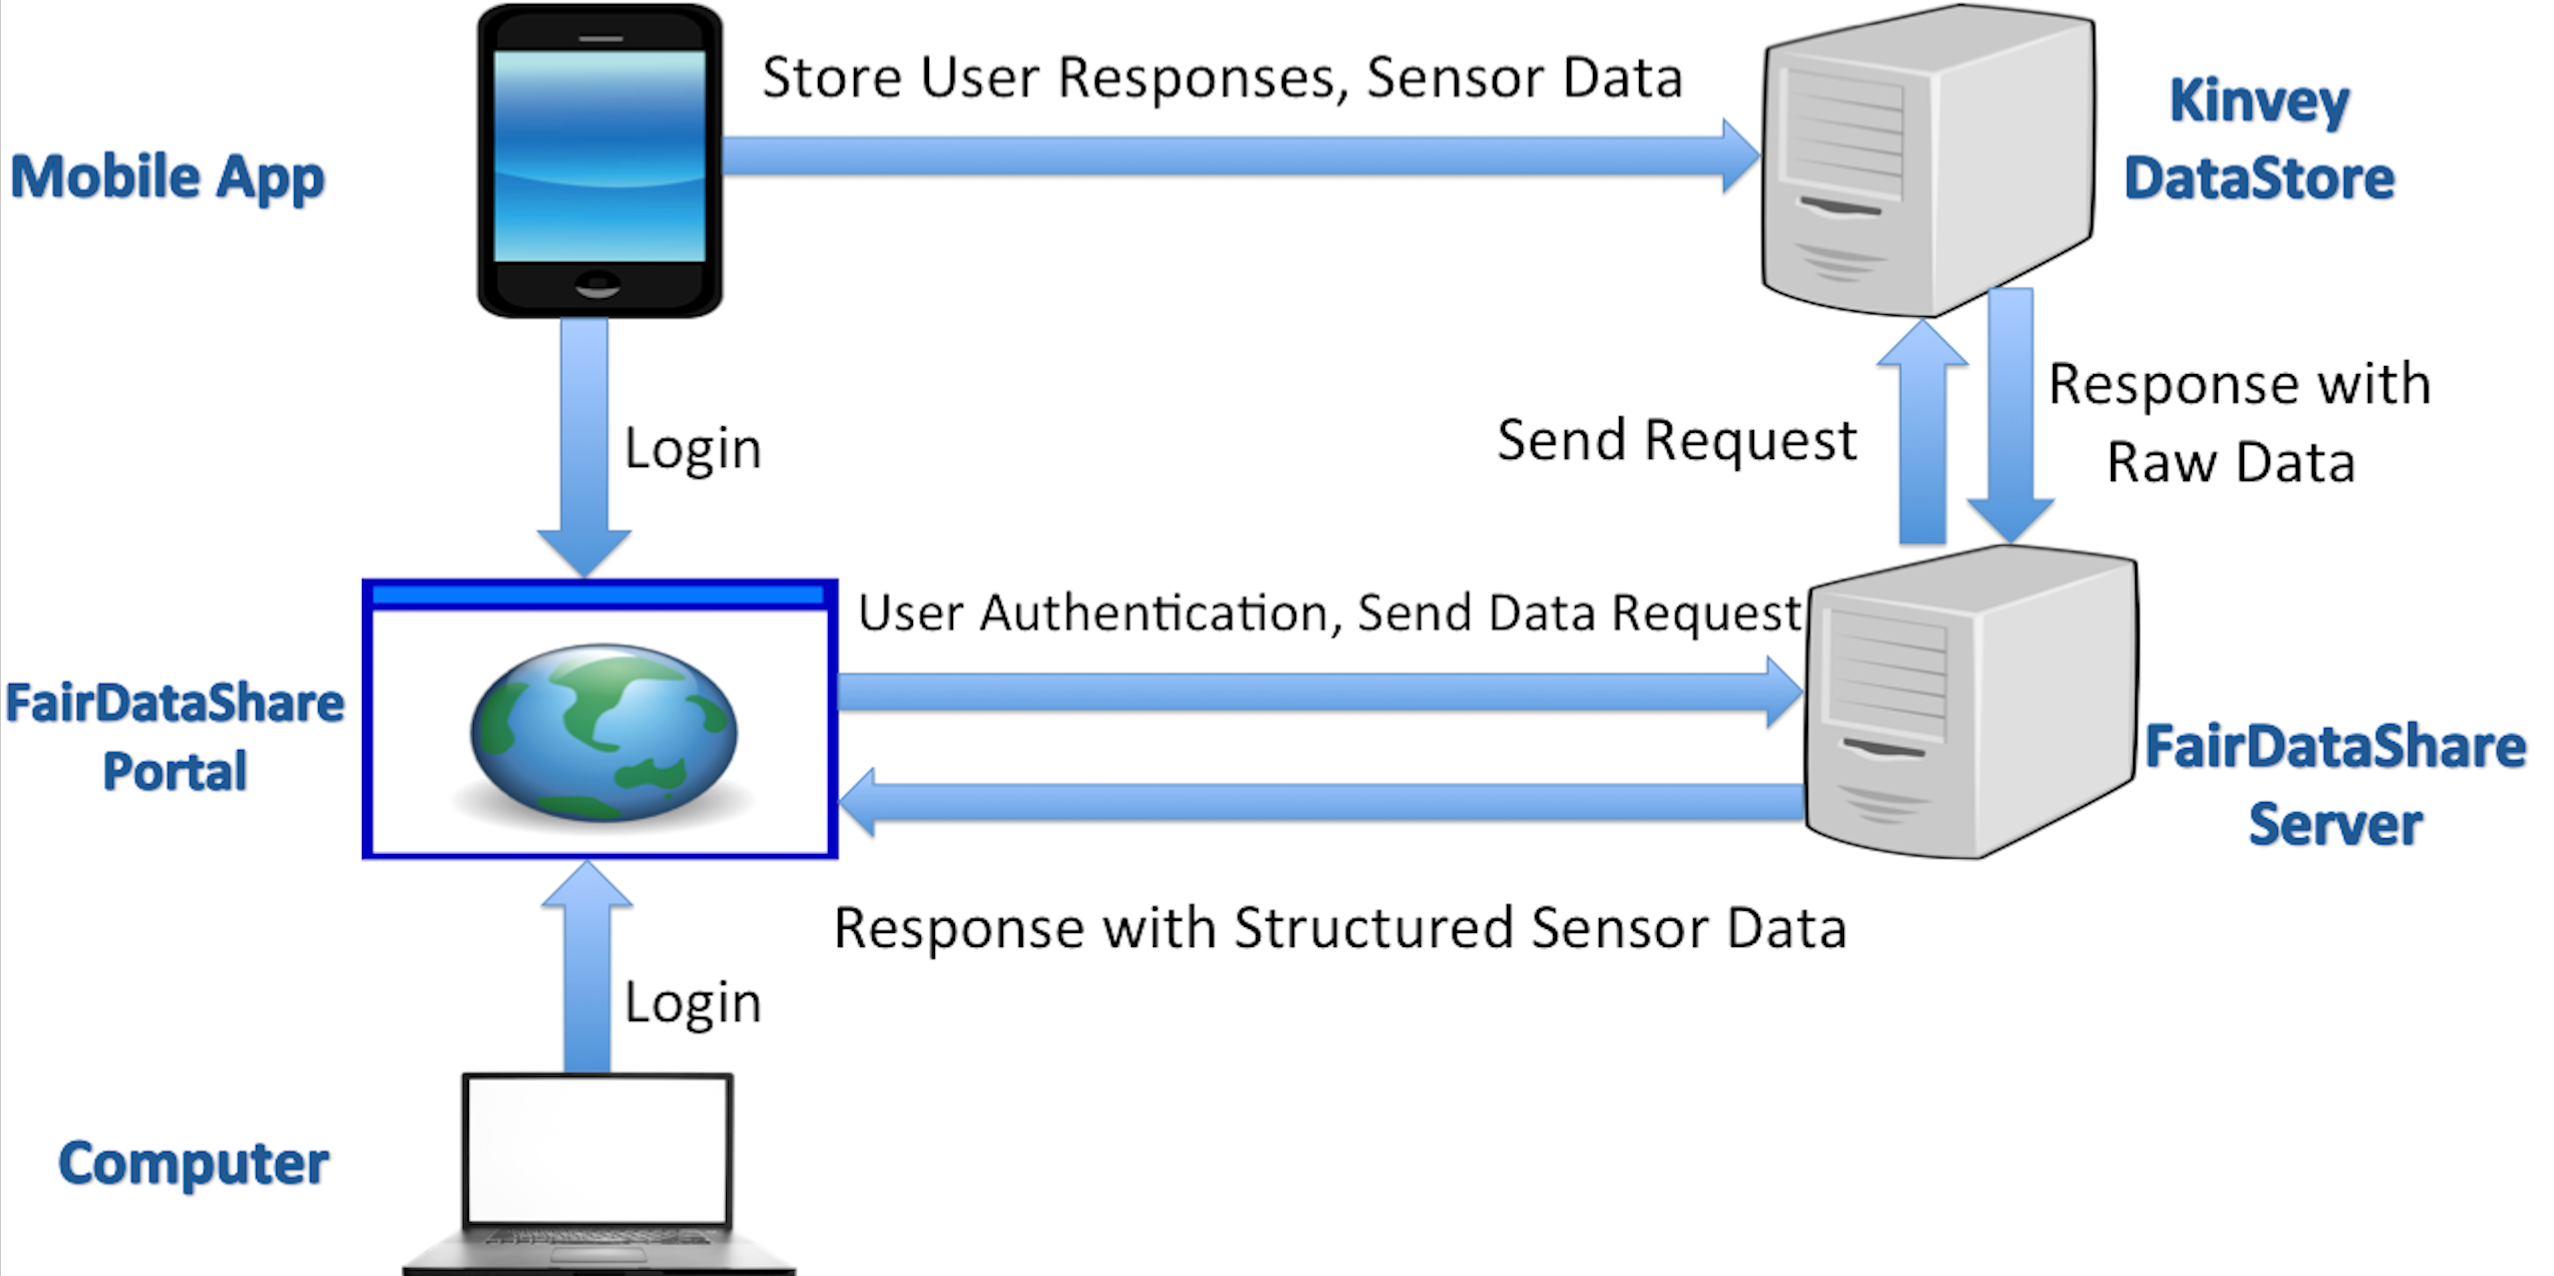
\includegraphics[width=\textwidth,keepaspectratio]{./images/blocks_app}
\caption{Conceptual Diagram of Mobile Application Architecture}
\label{fig:bb}
\end{figure}

The users can login into the FairDataShare Portal from their computer or the mobile application. Once the user is authenticated, the user requests
are sent from the FairDataShare server to the Kinvey Data Store\footnote{\url{https://kinvey.com}}. Kinvey in turn fetches the appropriate data and gives it back to the FairDataShare Server. This in turn structures the data so it can be readable, and pushes it to the user to see on the portal. The concept is similar for the Stakeholders, except they can only access the portal through the computer and not the mobile application.


\section{The Mobile Application}

The mobile application was developed for the Android platform with phones having API above level 17\footnote{\url{https://developer.android.com/guide/topics/manifest/uses-sdk-element.html}}. Phones are assumed to have internet connectivity and sufficient storage space of at least 100 Mb.
Below is an explanation of some of the tasks that take place in the application. A block diagram of the interaction of each of the components in the application is depicted in figure \ref{fig:chap5_app}.

\subsection{Local Storage} \label{loc}
The local storage is an integral part of the application. The database used is SQLite\footnote{\url{https://developer.android.com/reference/android/database/sqlite/package-summary.html}} and is the default database
for the Android environment. Small sized unrelated data pieces are stored in preference files (as key value pairs), whereas larger related
data is stored in the database. The following paragraphs will explain each table present in this application followed with 
their function and schema. All tables explained here are pertaining to the user using the mobile application and not the server.

\begin{figure}[ht!]
\centering
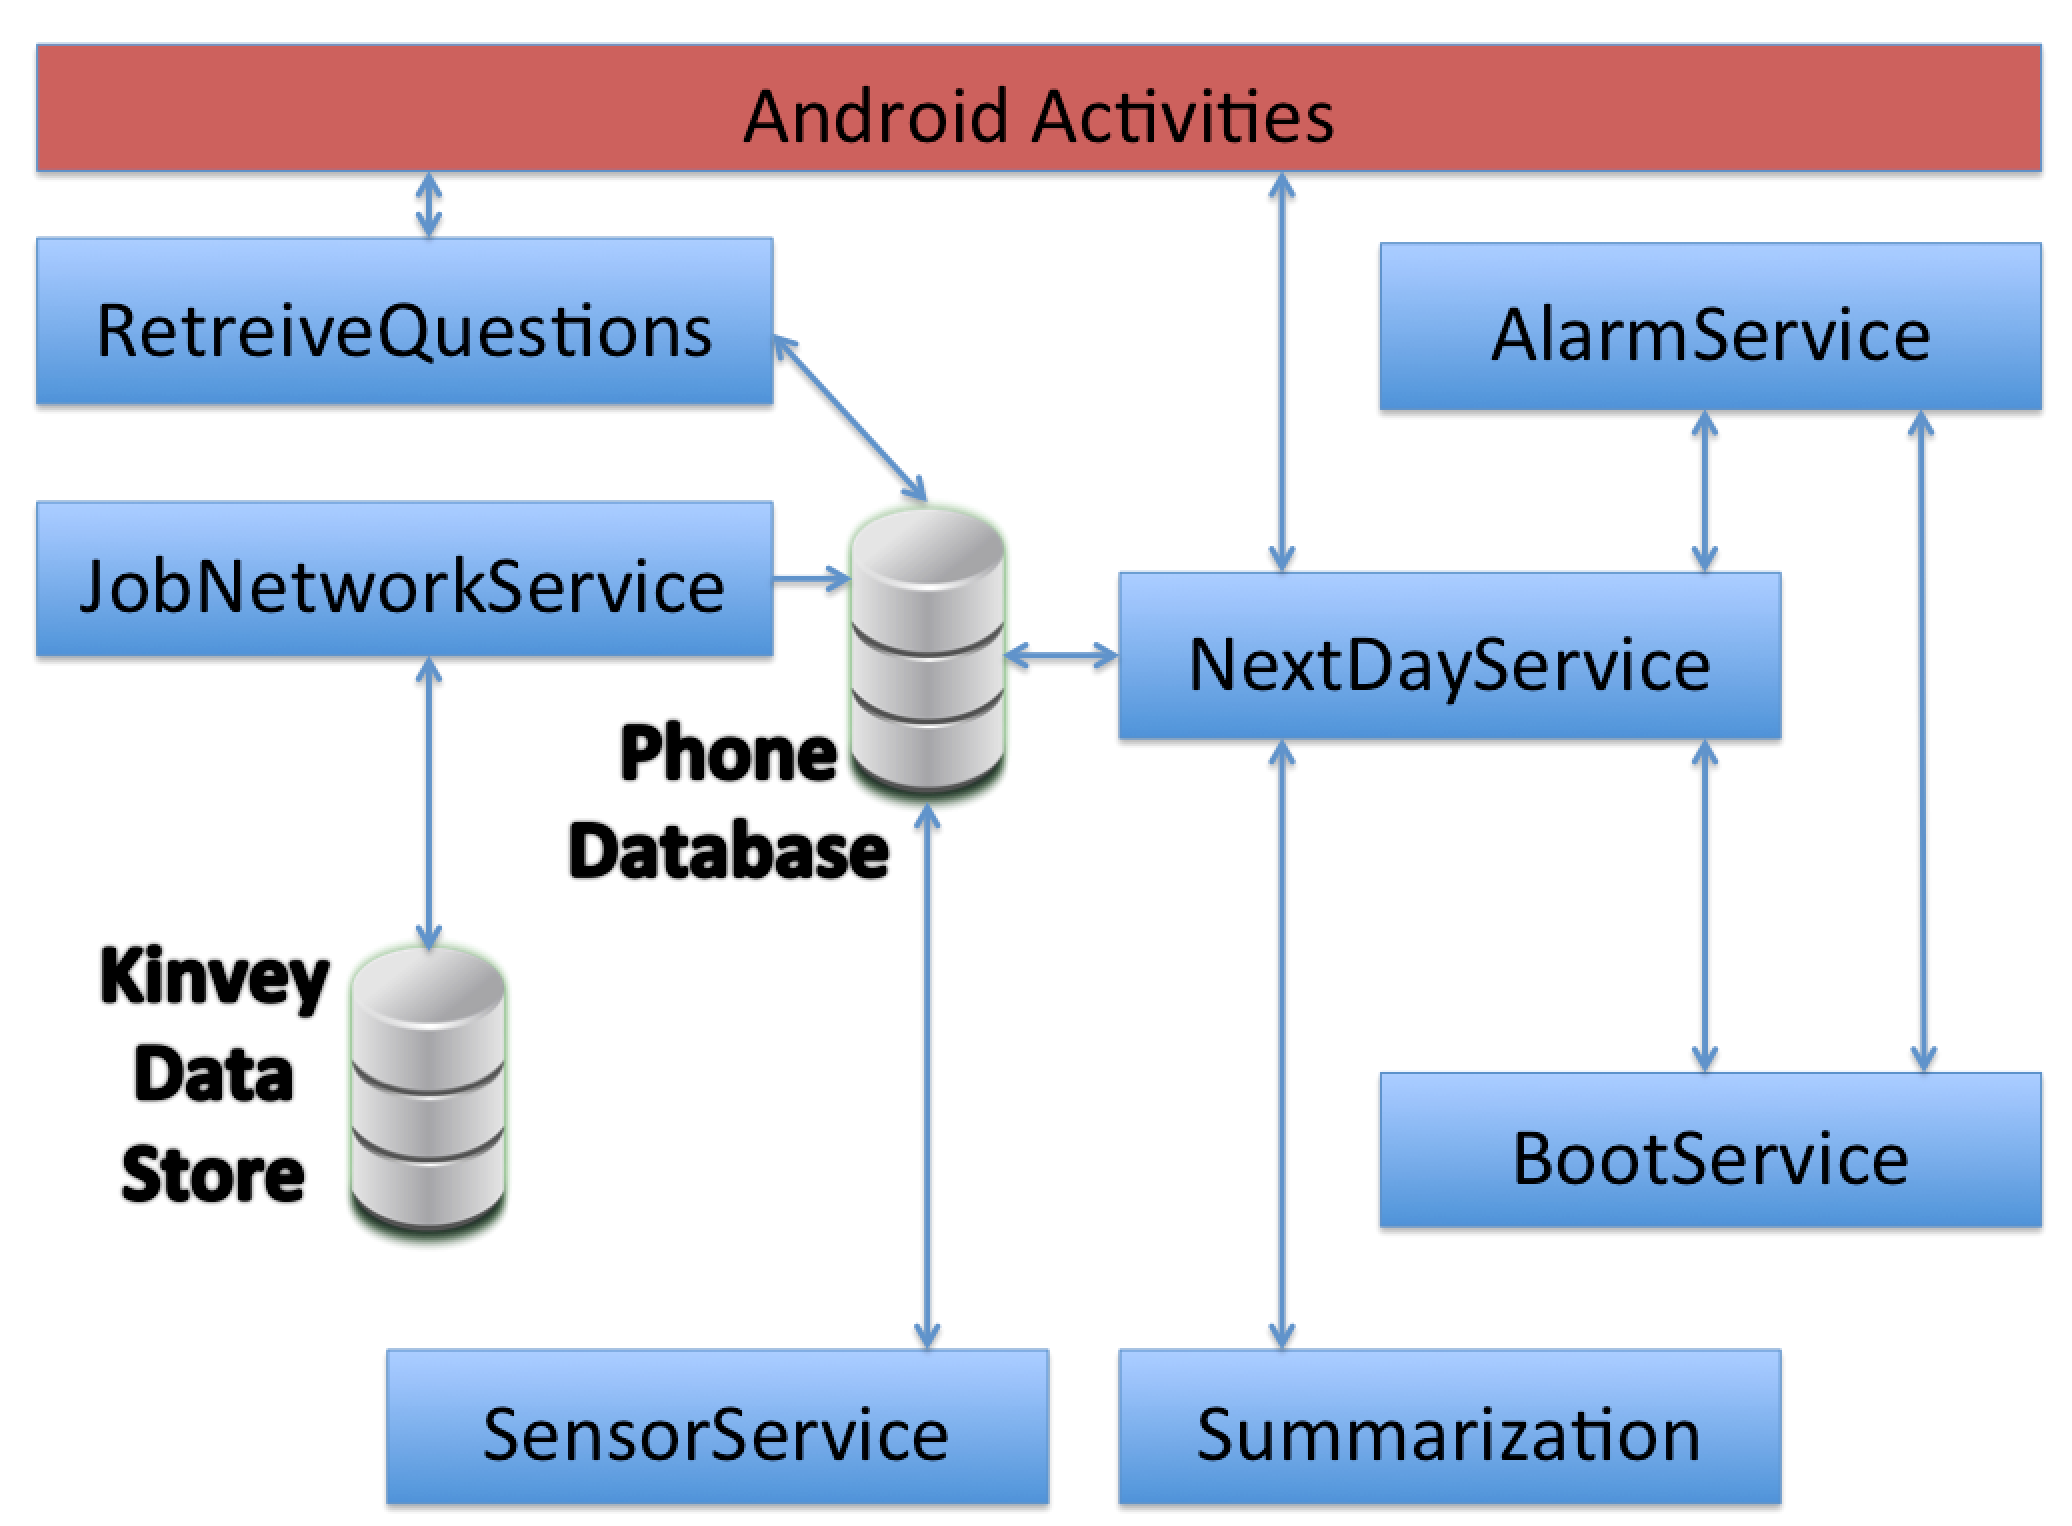
\includegraphics[width=\textwidth,height=0.6\textwidth]{./images/chap5_app}
\caption{Interaction of Components of Mobile Application}
\label{fig:chap5_app}
\end{figure}

\begin{figure}[htp]
\subtop[Table Schema of \texttt{QUESTION\_STORE}\label{fig:db_quest}]{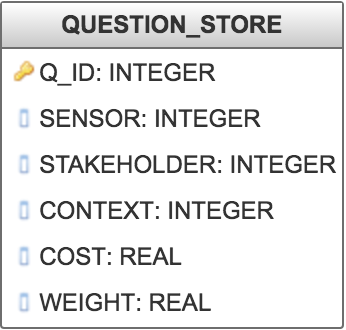
\includegraphics[width=0.4\linewidth]{./images/db_quest}}\hspace{1em}
\subtop[Table Schema of \texttt{WHICH\_ANSWERS}\label{fig:db_which}]{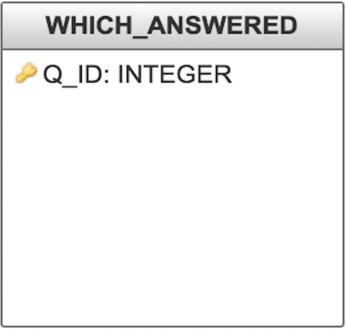
\includegraphics[width=0.4\linewidth]{./images/db_which_1}}
\caption{Table Schemas}
\label{fig:ts1}
\end{figure}


Figure \ref{fig:db_quest} shows the \texttt{QUESTION\_STORE's} table schema. This table stores each possible data request with its features such as with its sensor \textit{SENSOR}, stakeholder \textit{STAKEHOLDER} and context \textit{CONTEXT}. Each of these are represented by an integer, for example sensor 0 stands for accelerometer sensor. Each data request is accompanied by
an unique question identifier \textit{QID}, weight assigned \textit{WEIGHT} and the cost assigned \textit{COST}. This data is not sent to 
the server.

Figure \ref{fig:db_which} depicts the table \texttt{WHICH\_ANSWERS}'s table schema. This stores the questions identifier \textit{QID} of each data request that has
been answered by the user for each round. This is helpful while fetching data requests, so as not to fetch the request twice in the same round. It makes sure that all questions are answered before answering them for a second time. This data is not sent to the server.

\begin{figure}[htp]
\subtop[Table Schema of \texttt{STORE\_ANSWERS}\label{fig:db_ans}]{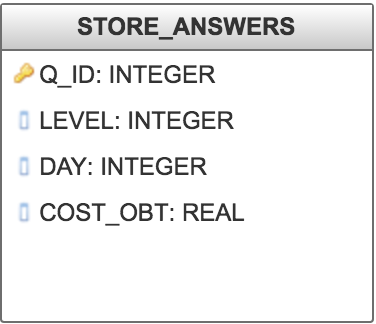
\includegraphics[width=0.4\linewidth]{./images/db_ans}} \hspace{1em}
\subtop[Table Schema of \texttt{STORE\_POINTS}\label{fig:db_points}]{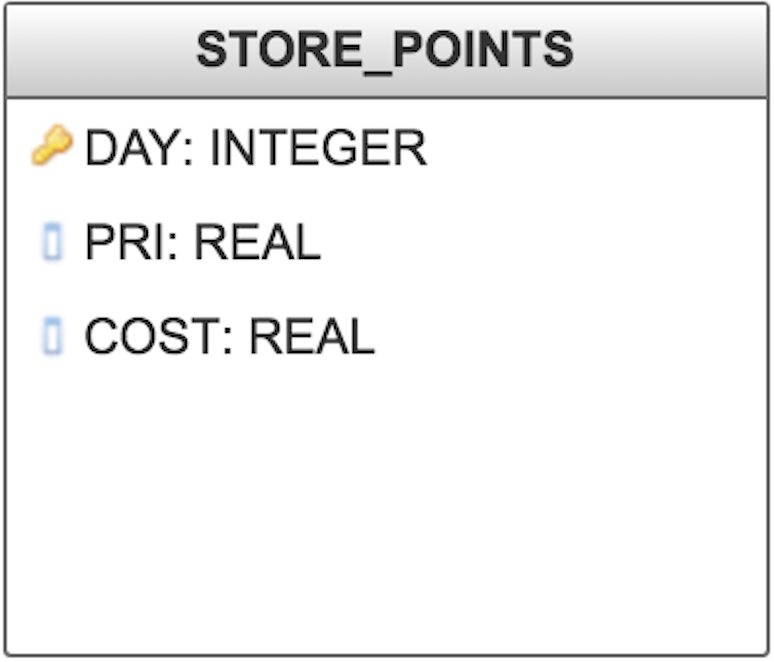
\includegraphics[width=0.4\linewidth]{./images/db_points}}
\caption{Table Schemas}
\label{fig:ts11}
\end{figure}

Figure \ref{fig:db_ans} explains the schema of \texttt{STORE\_ANSWERS} table. This table is used to store the data request identifier \textit{QID} with the corresponding
user responses \textit{LEVEL}, along with the increase or decrease in credit obtained \textit{COST\_OBT}. The total cost is calculated by adding all the costs in this table. Similarly, the total privacy is calculated by averaging of all the user responses stored in this table. Only the most recent responses are stored in this table. The content of the table is not sent over to the server.

Figure \ref{fig:db_points} denotes the schema of \texttt{STORE\_POINTS} table. This table is used to store the credit and privacy obtained for each bidding day.
This information is sent to the server as soon one bidding day is over.

\begin{figure}[ht!]
\centering
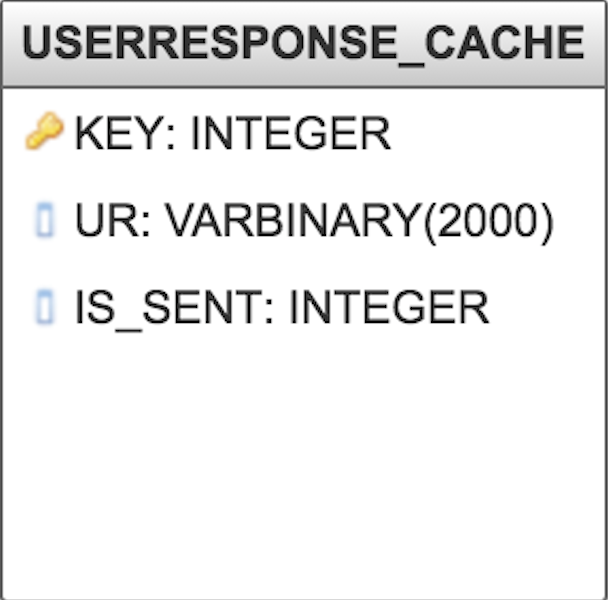
\includegraphics[width=0.4\linewidth]{./images/db_ur}
\caption{Table \texttt{USERRESPONSE\_CACHE} Schema}
\label{fig:db_ur}
\end{figure}

Figure \ref{fig:db_ur} depicts the \texttt{USERRESPONSE\_CACHE} tables's schema. This table stores a unique key \textit{KEY} for each user response, followed by a flag \textit{ISSENT}, which is 1 if the response is not sent to the server, and 0 if it is sent. The user response saved consists of the following entries :

\begin{enumerate}
	\item User Identifier
	\item Timestamp of the response
    \item Sensor Identifier
    \item Stakeholder Identifier
    \item Context Identifier
    \item Privacy Level response for this data request
    \item Cost obtained for this data request
    \item Current Total Privacy of the user
    \item Current Total Credit of the user
    \item Maximum Obtainable Credit for this data request in this round
    \item Metric Chosen to Improve  (Improve Privacy or Improve Credit)
\end{enumerate}

All of the above fields are packed into the field \textit{ur} shown in \ref{fig:db_ur}. The data in this table is sent to the server. Once the entry is sent to the server, the \textit{ISSENT} field is changed to 0 and deleted locally. The unique keys \textit{KEY} are useful for deleting sent entries. Figure \ref{fig:ts2} and \ref{fig:ts22} show the table schemas for data storage of the following sensors:

\begin{enumerate}
	\item Accelerometer in the \texttt{STORE\_ACCELEROMETER} table
	\item Noise in the \texttt{STORE\_NOISE}
    \item Location in the  \texttt{STORE\_LOCATION}
    \item Light in the  \texttt{STORE\_LIGHT}
\end{enumerate}

The general schema for all the sensor tables is the following :

\begin{enumerate}
	\item \textit{KEY} - Uniquely identifies each sensor entry
	\item \textit{TIMESTAMP} - The time the sensor value was collected
    \item \textit{ISSENT} - Denotes whether the sensor entry has been sent to the server or not
    \item The other columns are specific to each sensor and represent the actual sensor values collected 
\end{enumerate}

\begin{figure}[htp]
\subtop[Table Schema of \texttt{STORE\_ACCELEROMETER}\label{fig:db_acc}]{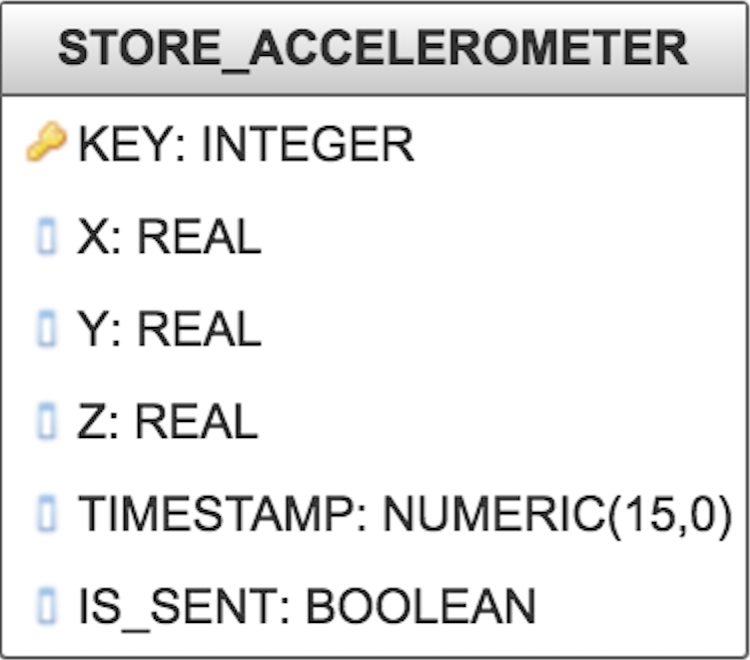
\includegraphics[width=0.4\linewidth]{./images/db_acc}}\hspace{1em}
\subtop[Table Schema of \texttt{STORE\_NOISE} \label{fig:db_noise}]{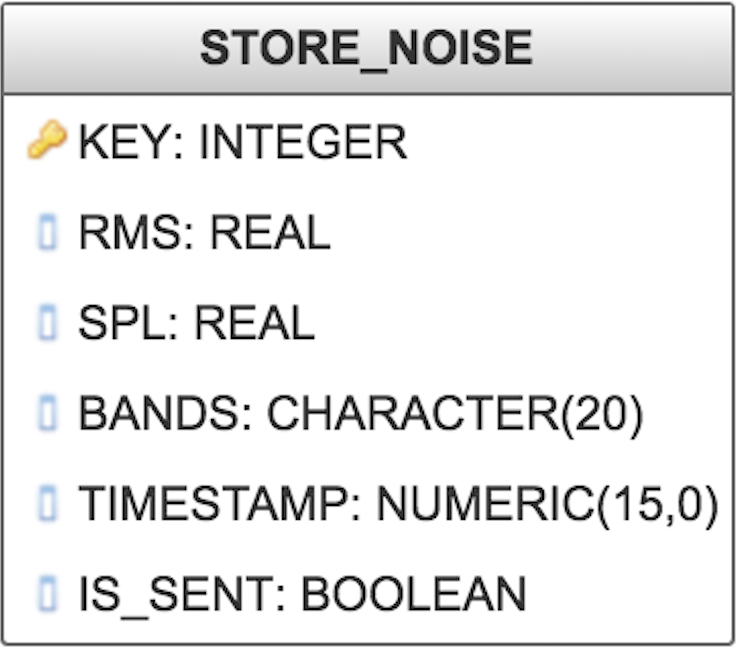
\includegraphics[width=0.4\linewidth]{./images/db_noise}}%
\caption{Table Schemas for Sensor Data}
\label{fig:ts2}
\end{figure}



\begin{figure}[htp]
\subtop[Table Schema of \texttt{STORE\_LOCATION}\label{fig:db_loc}]{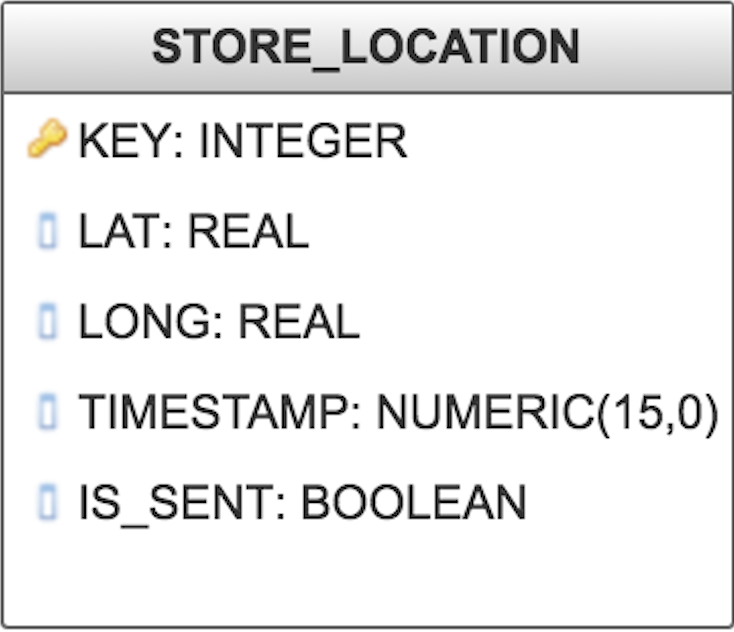
\includegraphics[width=0.4\linewidth]{./images/db_loc}}\hspace{1em}
\subtop[Table Schema of \texttt{STORE\_LIGHT} \label{fig:db_light}]{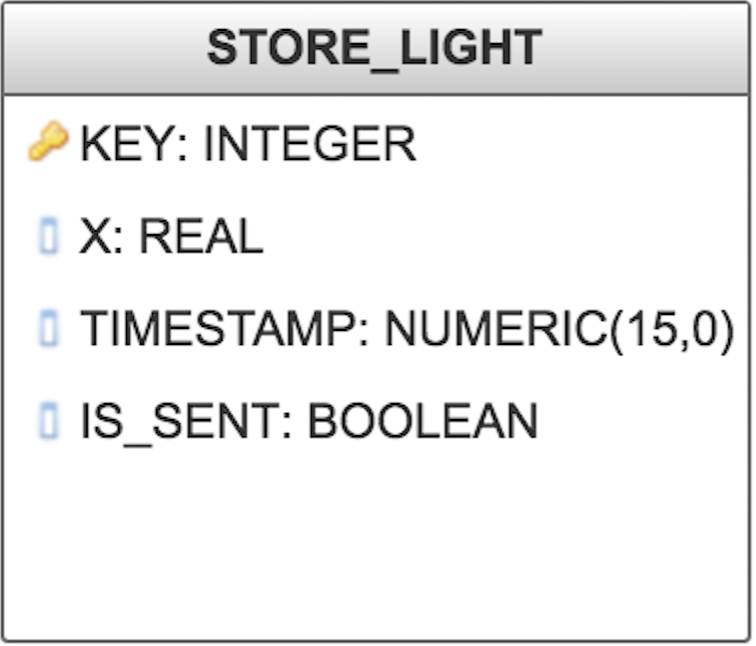
\includegraphics[width=0.4\linewidth]{./images/db_light}}%
\caption{Table Schemas for Sensor Data}
\label{fig:ts22}
\end{figure}

\subsection{Alarms and Notifications}

Every bidding day where the user answers data requests lasts for a period of 24 hours. After one bidding day is over, the system needs to be informed in a timely manner to perform some application critical functions. The functions performed are explained in detail in section \ref{next}. 
To inform the system of such an event Android provides the functionality in the form of alarms. 

Alarms can be set to go off just once or in a repeated fashion to trigger tasks. Unfortunately, the alarms provided by Android are not exact for some versions \footnote{\url{https://developer.android.com/training/scheduling/alarms.html}}, in the sense that they are triggered around that time set but not exactly at that time to optimize the battery, and can be delayed upto 24 hours. Hence, it is decided to set the repeating alarms manually. 

The first time the application opens the alarm is set to ring in exactly 24 hours, but things change when the phone is switched off.
One of the conditions of the experiment is not to have the phone switched off at any time. Nevertheless, it is taken into account the scenario where
the phone is kept switched off for a period of time. There are various things that can happen:

\begin{enumerate}
	\item The phone is rebooted.
	\item The phone is switched off, during this time an alarm is missed.
    \item The phone is switched off for a period greater than 24 hours. One or more alarms can be missed.
\end{enumerate}

Once the phone is switched off, all alarms are erased from memory \footnote{\url{https://developer.android.com/reference/android/app/AlarmManager.html}}. Alarms do not execute when the phone is switched off. Hence, when the phone switches on,
BootReceiver service of the application is triggered with pseudocode shown in \ref{boot}. This checks whether an alarm has been missed, if it has been missed 200 seconds is given for the phone to stabilize after boot before triggering tasks. Otherwise, a new alarm is set using the pseudocode shown in \ref{setalarm}. To set an alarm we need the time difference between now and when the alarm should ring. After that is calculated, the alarm is set.

\begin{algorithm}
\caption{BootService Algorithm}\label{boot}
\begin{algorithmic}[1]
\Procedure{BootService}{}
\State $\textit{now} \gets \text{current timestamp}$
\State $i \gets \text{timestamp of last triggered alarm}$
\If {$\textit{now}-i < 86400$}
  \State $\text{Call }\textit{SetAlarmLater()}$
\Else
  \State $\text{Set alarm in 200 seconds}$
\EndIf
\EndProcedure
\end{algorithmic}
\end{algorithm}


\begin{algorithm}
\caption{Alarm Algorithm}\label{setalarm}
\begin{algorithmic}[1]
\Procedure{SetAlarmLater}{}
\State $\textit{now} \gets \text{current timestamp}$
\State $i \gets \text{timestamp of last triggered alarm}$
\State $\textit{latertime} \gets \textit{i}+\text{86400}$
\State $\textit{latergap} \gets \textit{latertime}-\textit{now}$
\State $\text{Set Alarm in latergap seconds}$
\EndProcedure
\end{algorithmic}
\end{algorithm}

\subsubsection{Going to the Next Data Sharing Day} \label{next}
Once the alarm rings, it marks the end of a bidding day. Once a bidding day ends a number of tasks need to be executed
and for this the NextDayService is triggered, which is described in pseudocode shown in \ref{nextday}. To start with the the privacy and credit is sent to the server and stored locally in the \texttt{STORE\_POINTS} table. \textit{Privacy} which is the total privacy obtained, \textit{Credit} is the total credit obtained, \textit{Round} which is the number of times the user answered all the questions and \textit{CurrentQuestion} which is the current question the user is answering is all reset to zero. The \textit{Day} corresponds to the current day number is incremented by one to denote the next bidding day.

\begin{algorithm}
\caption{NextDayService Algorithm}\label{nextday}
\begin{algorithmic}[1]
\Procedure{NextDayService}{}
\State $\text{Store }\textit{Privacy, Credit, Day } \text{in } \textit{STOREPOINTS}$
\State $\text{Send }\textit{Privacy, Credit, Day } \text{to Server}$
\State $\textit{Privacy, Credit, Round, CurrentQuestion} \gets \text{0}$
\State $\textit{Day} \gets \textit{Day}+1$
\State $\text{Store current time}$
\State $\text{Call }\textit{Summarization()}$
\If {$\textit{Day} > \textit{End}$}
  \State $\text{End experiment}$
\Else
  \State $\text{Update user interface elements}$ 
\EndIf
\EndProcedure
\end{algorithmic}
\end{algorithm}

The current time of executing the alarm is saved in case the phone is rebooted or switched off. After that, the sensor data which is saved locally
needs to be summarized, the corresponding method is called and is explained in pseudocode shown in \ref{sum}. Finally it needs to be to checked if the experiment is over or not and update the user interface accordingly. This means either the various metrics on the improvement and bidding screens (which ever is currently active) are updated, or
the end of experiment screen is shown.

\subsection{Fetching Data Requests} \label{data_req}
A data requests need to be fetched from the database in two scenarios :

\begin{enumerate}
	\item After a question has been answered in the first bidding day (entry phase)
	\item After the privacy or credit improvement button has been clicked (core phase)
\end{enumerate}

In the first bidding day, once a data request has been answered the next one is fetched sequentially from the database. This just requires knowing the current data request number and fetching the next data request from table \texttt{QUESTION\_STORE}. For the other bidding days, fetching of the data requests depends on the improvement button chosen. According to the choice, the following is done:

\begin{enumerate}
	\item \textbf{Improve Privacy} - Obtain data request from table \texttt{STORE\_ANSWERS} where user has answered with lowest privacy
	\item \textbf{Improve Credit} - Obtain data request from table \texttt{STORE\_ANSWERS} where user has answered with highest privacy
\end{enumerate}

In addition to sending the data request to the user interface, it is needed to show how choosing each option of the data request will affect the total privacy and total credit metrics. To do this for the total cost, the computation $last-possible$ is output, where $last$ stands for the credit obtained the last time the data request was answered. $possible$ stands for the maximum amount of credit that can be obtained for this option (each data request has five privacy options \ref{o}). The possible total cost changes are shown under the options. For more detail on how credits are split among options in a data request refer \ref{options}.

Every option of a data request has an associated percentage of data that is given away as described in \ref{o}. According to the percentage of data given away, the total privacy is calculated for each possible option. The difference between the current privacy and each possible total privacy is calculated and indicated under each option. This gives an indication to the user as to what each option will do to the metrics.

\subsection{Recording User Choices}

The figure \ref{fig:db_ur} describes the table \texttt{USERRESPONSE\_CACHE}. Each time a user enters a response to a data request, all the fields mentioned in section
\ref{loc} are recorded and stored in a class object. This object is transformed into a byte array so as to be stored easily in the table as is without transformation.
When the JobNetworkService described in \ref{job} is called, the class object is sent as it is to the server after converting it back to an object.


\subsection{Sensor Data Collection and Summarization} 

Sensor data is collected from the following sensors :

\begin{enumerate}
	\item Accelerometer sensor
	\item Noise sensor
    \item Location sensor
    \item Light sensor
\end{enumerate}

A sensor service is triggered when the application is installed and is stopped when the experiment is over. This collects data from every sensor
every 30 seconds and stores it in the appropriate tables mentioned in section \ref{loc}.
At the end of a bidding day, sensor data needs to be summarized according to the wishes of the user. This starts by first finding out the lowest privacy level for each sensor. Privacy levels range from one to five, that is from the lowest to highest privacy levels. Using this level
summarization is done as shown in pseudocode \ref{sum}. Every privacy level corresponds to an action:

\begin{enumerate}
	\item 1- All data is sent to the server
	\item 2- Send 75\% of the data
    \item 3- Send 50\% of the data
    \item 4- Send 25\% of the data
    \item 5- Do not send any data
\end{enumerate}

Initially all the sensor data has a field \textit{ISSENT} with value of zero. Data that should be sent to the server is set with $\textit{ISSENT}=1$, and all others that have value $\textit{ISSENT}=0$ are ignored.

\begin{algorithm}
\caption{Summarization Algorithm}\label{sum}
\begin{algorithmic}[1]
\Procedure{Summarization}{}
\For{$\text{each sensor}$}
\State $\text{Fetch sensor data from } \textit{sensor table}$
\State $\textit{level} \gets \text{Fetch user privacy level}$
\If {$\textit{level} \gets 1$}
  \State $\text{Set all } \textit{ISSENT} \gets \text{1}$
\ElsIf {$\textit{level} \gets 2$}
	\For{$\text{3 out of every 4 records}$}
 	 \State $\textit{ISSENT} \gets \text{1}$
 	\EndFor 
\ElsIf {$\textit{level} \gets 3$}
  \For{$\text{1 out of every 2 records}$}
 	 \State $\textit{ISSENT} \gets \text{1}$
 	\EndFor
\ElsIf {$\textit{level} \gets 4$}
  \For{$\text{1 out of every 4 records}$}
 	 \State $\textit{ISSENT} \gets \text{1}$
 	\EndFor
\EndIf
\State $\text{Delete all entries with } \textit{ISSENT} \gets 0$
\State $\text{Update Database}$
\EndFor
\EndProcedure
\end{algorithmic}
\end{algorithm}

\subsection{Server Synchronization} \label{job}

User responses and sensor data need to be sent to the server. This is done periodically every 5000 seconds in order to free up space on the phone whenever the internet is available. It is triggered first when the application is started for the first time. Data is fetched from the tables in the database. Data with fields marked as $\textit{ISSENT}=1$ is data that is ready and that has not been sent yet to the server. Such data is sent, and when an acknowledgement is received from the server, this data is deleted from the table.

\begin{algorithm}
\caption{JobNetworkService Algorithm}\label{nextday}
\begin{algorithmic}[1]
\Procedure{NetworkService}{}
\State $ \text{Fecth data from } \textit{USERRESPONSECACHE}$
 \For{$\text{each record}$}
 	 \If {$\textit{ISSENT} == \textit{1}$}
  \State $\text{Send record to Server}$
  \If {$\text{SUCCESS}$}
  \State $\text{Delete record}$  
  \EndIf
  \EndIf
 	\EndFor

\For{$\text{each sensor}$}
 	 \State $ \text{Fecth data from } \textit{sensor table}$
 	  \For{$\text{each record}$}
 	 \If {$\textit{ISSENT} == \textit{1}$}
  \State $\text{Send record to Server}$
  \If {$\text{SUCCESS}$}
  \State $\text{Delete record}$  
  \EndIf
  \EndIf
 	\EndFor
	
 	\EndFor
\EndProcedure
\end{algorithmic}
\end{algorithm}



\section{The Server}

\subsection{Kinvey Data Storage}

Kinvey \footnote{\url{http://kinvey.com/}} is a mobile backend as a service which provides a platform for mobile phones to link applications to a backend cloud storage \footnote{\url{https://en.wikipedia.org/wiki/Mobile_backend_as_a_service}}. For the purpose of this application the backend has been used to store data and for some business logic implementations in javascript.

\subsubsection{Security}

All communications from the application to the server is encrypted using TLS/SSL encryption \footnote{Kinvey white paper : KINVEY CLOUD
SERVICE: SECURITY
OVERVIEW 2014} to communicate with the backend service. This is automatically provided and done by the Kinvey SDK.

\subsubsection{Collection Store}

Locally, all information is stored in SQLite which is a relational database. The database used in Kinvey is MongoDB so instead we have collections 
on the server.
When the user starts the application, general personal information is entered as explained in \ref{loc}. This data is stored in the
collection UserInformation with the schema shown in the screen shots \ref{fig:col_ui_1} and \ref{fig:col_ui_2}.

Once this is done, users have to categorize the various Features, Sensors, Stakeholders and then the various Contexts. This information is sent to the server in collections named Features, Sensors, Stakeholders and Contexts. Schema is shown in \ref{fig:col_f}, \ref{fig:col_s}, \ref{fig:col_ss} and \ref{fig:col_c} respectively.

All the data stored locally on the mobile phone which is sent by the JobNetworkService explained in section \ref{job} is received by Kinvey.
User responses are stored in the collection UserResponse shown in \ref{fig:col_ur_1} and \ref{fig:col_ur_2}.

The sensor data sent by the JobNetworkService is stored in collections named after the sensors themselves. The schema of the tables
is shown in figures \ref{fig:col_loc}, \ref{fig:col_acc}, \ref{fig:col_light} and \ref{fig:col_noise}.

To keep track of all the existing users in the experiment, the collection Users stores all unique user identification strings of participants.
The schema is shown in \ref{fig:col_users}.

Finally, the collection Score shown in \ref{fig:col_score} stores the total privacy, total credit obtained by the user for each bidding day.

\subsubsection{Bussiness Logic} \label{bl}
Most of the bussiness logic used for the FairDataShare portal is present in Kinvey. There are two main scripts stored in Kinvey are:

\begin{enumerate}
    \item Script to find the privacy preferences of the users
    \item Script to perform data summarization \ref{sum}
\end{enumerate}

The stakeholders make a request for data on the FairDataShare portal giving the following details:

\begin{enumerate}
    \item Bidding day number
    \item Anonymous user
    \item Sensor
    \item Context
\end{enumerate}

Given this input plus the category of the stakeholder (which is known from their registration), we look into the UserResponse Collection trying to find the most recent record that
fits this criteria and extract the privacy level.

Once the privacy level is known, summarization on user data is performed. Data has been taken from the user with a certain summarization, and if the summarization level is lower than the privacy level extracted, further summarization needs to be done. The pseudocode is shown in \ref{sum1}.

\begin{algorithm}
\caption{Server Summarization Algorithm}\label{sum1}
\begin{algorithmic}[1]
\Procedure{Summarization}{}
\State $\textit{data} \gets \text{sensor data from collection}$
\If {$\textit{summarizationlevel} == \textit{privacylevel}$}
	\State $\textbf{Return }\textit{data}$
\Else
	\State $\textit{skip} \gets \textit{summarizationlevel}-\textit{privacylevel}+1$
	 \For{$\text{every }\textit{skip} \text{number records out of 4}$}
 	 \State $\text{Delete record from}\textit{ data}$
 	 \EndFor
\EndIf
\State $\text{Return data to portal}$
\EndProcedure
\end{algorithmic}
\end{algorithm}

\subsection{FairDataShare Web Portal}
The FairDataShare portal makes use of a server at ETH Zurich other than the Kinvey Data Store to safely store the usernames, passwords of the users and the stakeholders in a collection. The database technology used is MongoDB. The language used to interact with Kinvey is Express.js, which is based on Node.js. Most of the data portal business logic is on Kinvey as described in section \ref{bl}. The webpage was constructed using simple Html and css. All screenshots of the portal including detailed information is provided in chapter \ref{exp}.









